% !TeX root = ./../../main.tex
% Interferencja jednokubitowa, wersja zwarta rysunku fig:tb01:bloch (zadanie PHD-TS-95, 2026-11-27):
% (a) obwód H - P(phi) - H z pomiarem,
% (b) prawdopodobieństwa wyników w funkcji fazy lokalnej:
%     p(0) = (1 + cos phi)/2, p(1) = (1 - cos phi)/2 oraz p(0) = (1 + v cos phi)/2 dla v = 0,6 (stłumione koherencje).
% Wersja pełna, ze sferą Blocha, jest w pliku tb01_interference.tex.
\begin{subfigure}[c]{0.36\textwidth}
  \centering
  \begin{quantikz}[column sep=0.25cm]
    \lstick{$\ket{0}$} & \gate{\mathrm{H}} & \gate{\mathrm{P}(\varphi)} & \gate{\mathrm{H}} & \meter{}
  \end{quantikz}
  \caption{}\label{fig:tb01:interference:circuit}
\end{subfigure}\hfill
\begin{subfigure}[c]{0.6\textwidth}
  \centering
  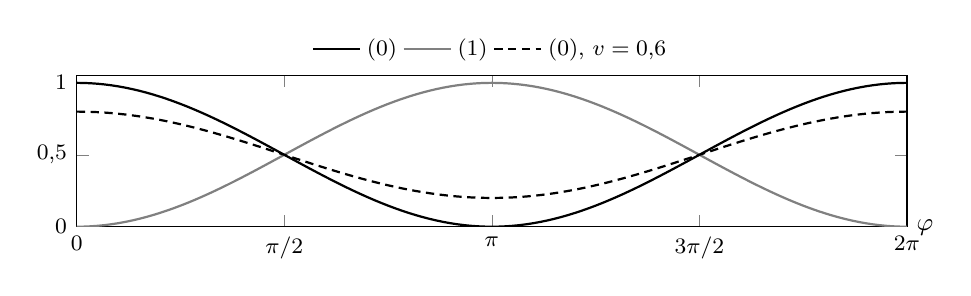
\begin{tikzpicture}
    \begin{axis}[
        width=\linewidth, height=3.5cm,
        xmin=0, xmax=6.2832, ymin=0, ymax=1.05,
        xtick={0,1.5708,3.1416,4.7124,6.2832},
        xticklabels={$0$,$\pi/2$,$\pi$,$3\pi/2$,$2\pi$},
        ytick={0,0.5,1},
        yticklabels={$0$,$0{,}5$,$1$},
        xlabel={$\varphi$}, xlabel style={at={(1,0)}, anchor=north west, yshift=6pt},
        legend style={font=\footnotesize, at={(0.5,1.03)}, anchor=south, draw=none, legend columns=3},
        tick label style={font=\footnotesize}, label style={font=\small},
        samples=121, domain=0:6.2832,
      ]
      \addplot[thick, black] {(1+cos(deg(x)))/2};
      \addlegendentry{$\prob(\ket{0})$}
      \addplot[thick, gray] {(1-cos(deg(x)))/2};
      \addlegendentry{$\prob(\ket{1})$}
      \addplot[thick, black, densely dashed] {(1+0.6*cos(deg(x)))/2};
      \addlegendentry{$\prob(\ket{0})$, $v=0{,}6$}
    \end{axis}
  \end{tikzpicture}
  \caption{}\label{fig:tb01:interference:plot}
\end{subfigure}
